\documentclass[11pt,]{article}
\usepackage{lmodern}
\usepackage{amssymb,amsmath}
\usepackage{ifxetex,ifluatex}
\usepackage{fixltx2e} % provides \textsubscript
\ifnum 0\ifxetex 1\fi\ifluatex 1\fi=0 % if pdftex
  \usepackage[T1]{fontenc}
  \usepackage[utf8]{inputenc}
\else % if luatex or xelatex
  \ifxetex
    \usepackage{mathspec}
  \else
    \usepackage{fontspec}
  \fi
  \defaultfontfeatures{Ligatures=TeX,Scale=MatchLowercase}
    \setmainfont[]{Arial}
\fi
% use upquote if available, for straight quotes in verbatim environments
\IfFileExists{upquote.sty}{\usepackage{upquote}}{}
% use microtype if available
\IfFileExists{microtype.sty}{%
\usepackage{microtype}
\UseMicrotypeSet[protrusion]{basicmath} % disable protrusion for tt fonts
}{}
\usepackage[margin=.5in]{geometry}
\usepackage{hyperref}
\hypersetup{unicode=true,
            pdfborder={0 0 0},
            breaklinks=true}
\urlstyle{same}  % don't use monospace font for urls
\usepackage{natbib}
\bibliographystyle{plainnat}
\setlength{\emergencystretch}{3em}  % prevent overfull lines
\providecommand{\tightlist}{%
  \setlength{\itemsep}{0pt}\setlength{\parskip}{0pt}}
\setcounter{secnumdepth}{5}

%%% Use protect on footnotes to avoid problems with footnotes in titles
\let\rmarkdownfootnote\footnote%
\def\footnote{\protect\rmarkdownfootnote}


  \title{}
    \author{}
    \date{}
  

%%%%%%%%%%
% personal preamble edits here
%%%%%%%%%%
\pagenumbering{gobble}

% can toggle this for Helvetica
%\usepackage{helvet}
%\renewcommand{\familydefault}{\sfdefault}

% \titlespacing*{\paragraph}{0pt}{2pt}{1em}

% set section numbering/lettering
% tips for seccntformat: https://tex.stackexchange.com/questions/95896/how-to-format-subsection-title-without-packages
\makeatletter
\def\@seccntformat#1{%
  \expandafter\ifx\csname c@#1\endcsname\c@section\else
  \expandafter\ifx\csname c@#1\endcsname\c@paragraph\else
  \csname the#1\endcsname\quad
  \fi\fi}
  
  % stucture for these commands: https://texfaq.org/FAQ-atsigns
  \renewcommand\section{
  \@startsection{section}{1}{\z@}
    {-3.5ex \@plus -1ex \@minus -.2ex}
    {1.0ex \@plus.2ex} %reduce space below section (was 1.5ex)
    {\normalfont\normalsize\bf\uppercase}} %modify font style
    
  \renewcommand\subsection{
  \@startsection{subsection}{2}{\z@}
    {-1.5ex\@plus -1ex \@minus -.2ex}%reduce space above subsection (was -3.25ex)
    {0.5ex \@plus .2ex}%reduce space below subsection (was 1.5ex)
    {\normalfont\normalsize\bf}} %modify font style
    
  \renewcommand\subsubsection{
  \@startsection{subsubsection}{3}{\z@}
    {-1.0ex\@plus -1ex \@minus -.2ex}%reduce space above subsubsection (was -3.25ex)
    {0.5ex \@plus .2ex}%reduce space below subsubsection (was 1.5ex)
    {\normalfont\normalsize\bf}} %modify font style
    
  \renewcommand\paragraph{
  \@startsection{paragraph}{4}{\z@}
    {-0.5ex\@plus -1ex \@minus -.2ex}%reduce space above paragraph (was -3.25ex)
    {-1.5ex \@plus .2ex}%convert space below paragraph to an indent (was 1.5ex)
    {\normalfont\normalsize\bf}} %modify font style    
\makeatother

\renewcommand\thesubsection{\Alph{subsection}.}
\renewcommand\thesubsubsection{\thesubsection\arabic{subsubsection}.}

% reduce spacing at the top of lists
\usepackage{enumitem}
\setlist{topsep = 2pt}

% allow text to wrap around figures
\usepackage{graphicx}
\usepackage{wrapfig}

%%%%%%%%%%

\begin{document}

\section{Specfic Aims}\label{specfic-aims}

The potential of real-world evidence from electronic health records
(EHRs) and claims data to inform regulatory decision-making is currently
being assessed (\cite{article1}). They are both important sources of
electronic data that can be utilized for health services research and
quality-of-care evaluations. Claims data have been utilized for research
purposes for many years, but EHRs, due to their high level of detail,
are gaining in popularity. While each data source has its own benefits,
combining the two sources can create a synergy that is useful for
research and policy applications. The ability to match EHR with
insurance claims data has the potential to revolutionize the way patient
care is analyzed and evaluated. EHR and claims data each provide only
partial information about a patient's health journey, and integrating
these sources of information provides a more comprehensive view of a
patient's health status. The main purpose of claims data is to bill and
pay for health services, while EHRs are designed for managing and
recording patient care. However, the current process of matching EHR and
claims data is time-consuming and prone to errors. Automating this
process using machine learning and deep learning methods can improve the
accuracy and efficiency of matching, reducing the time and effort
required and improving healthcare overall (\cite{article2}).

A study sponsored by the Agency for Healthcare Research and Quality
(AHRQ) examined the process and outcome of combining administrative
claims data and EHRs from a state Medicaid population and an academic
medical center. The study group found that despite some challenges in
merging and analyzing claims and clinical data, the combination of both
sources of healthcare data produced a stronger analytic resource than
either source alone, and should be further evaluated and improved.

Therefore, our project will focus on matching EHRs and claims data with
the following specific aims:

\paragraph{Specific Aim 1: To develop a user-friendly web application
using R Shiny that enables users to capture new checks, add notes, and
navigate between
matches.}\label{specific-aim-1-to-develop-a-user-friendly-web-application-using-r-shiny-that-enables-users-to-capture-new-checks-add-notes-and-navigate-between-matches.}

The upcoming version of the web application is set to undergo major
enhancements, particularly in its front-end, which will incorporate new
and improved features to optimize the workflow and provide a better user
experience. The primary goal of these updates is to identify and resolve
any existing issues in the current system while introducing novel
features, such as next and previous match buttons, a check capture
function, a notes text box, and an error resolution function. The
addition of next and previous match buttons is intended to facilitate
quicker navigation between matches in the application, thus improving
the user's ability to move through the data with ease. The check capture
function will enable users to effortlessly capture and store checks
within the web application, streamlining the record-keeping process. The
notes text box feature will provide users with a handy way to better
understand the data columns, enabling them to perform more comprehensive
analyses. Furthermore, an error resolution function will be introduced
to help users quickly resolve any issues that may arise while using the
app. To develop these new features, an experimental approach will be
employed, involving the incorporation of new elements into the existing
R Shiny application. Overall, these enhancements aim to optimize the
application's functionality, streamline the workflow, and provide a more
user-friendly experience.

\paragraph{Specific Aim 2: To develop a matching algorithm using machine
learning and deep learning methods that can match EHRs with insurance
records.}\label{specific-aim-2-to-develop-a-matching-algorithm-using-machine-learning-and-deep-learning-methods-that-can-match-ehrs-with-insurance-records.}

By automating the matching process, the accuracy and efficiency of
matching will improve, reducing the time and effort required and
improving healthcare overall.To accomplish this aim, the first step will
involve cleaning and preprocessing the data to ensure its quality and
suitability for the algorithm. The data will then be split into train,
validate, and test sets to enable effective training and testing of the
algorithm. Traditional machine learning models and deep learning models
will be developed and trained to match EHRs with insurance records.
Performance evaluation will be conducted using various accuracy and
ROC/AUC metrics to determine the most effective model. An experimental
approach will be employed to improve the performance of the algorithm.
This will involve fine-tuning the models to enhance their accuracy and
efficiency, as well as testing them on larger datasets to determine
scalability. The development of a matching algorithm using machine
learning and deep learning methods is expected to significantly enhance
the accuracy and efficiency of matching EHRs with insurance records,
ultimately reducing the time and effort required for the process. This
will enable healthcare providers to concentrate on delivering
high-quality care to their patients, thereby improving healthcare
outcomes by minimizing errors and streamlining the healthcare delivery
process.

\section{Research Strategy}\label{research-strategy}

\subsection{Significance}\label{significance}

The ability to match electronic health records (EHR) with insurance
claims data is an innovative approach that has the potential to
revolutionize the way patient care is analyzed and evaluated. This is
because EHR and claims data each provide only partial information about
a patient's health journey, and integrating these sources of information
provides a more comprehensive view of a patient's health status.

EHR data provides robust information on demographics, diagnoses,
encounters, laboratory results, procedures, and medication orders.
However, it does not reflect activity outside of the care setting, such
as prescription fills, and is incomplete for patients who receive care
at multiple hospitals. On the other hand, medical and prescription
claims provide a continuous clinical story that represents care across
providers and inclusive of pharmacy transactions. Claims data also
captures costs and assesses medication compliance, but is short on
clinical detail and lacks lab values, tumor staging information, and
physicians' notes.

The integration of EHR and claims data offers health administrators,
researchers, and policy makers an opportunity to draw insights from the
richest versions of patient health data. By using clinical data from the
EHR, condition identification can be significantly improved. For
example, lab result data elements can support the identification of
people with chronic kidney disease even without a coded diagnosis.
Similarly, vital sign data can help identify people with hypertension
despite the lack of a claim-based diagnosis. There are various data
elements available in the EHR that, when analyzed, can allow the
identification of a condition that was either not recognized or not
coded for by the physician. EHR data enables better condition
identification by providing access to data elements that allow one to
impute a diagnosis, even if that diagnosis was never made.

Claims-linked EHR data offers integrated evidence with a fuller
representation of reality and helps researchers follow the full story of
a subject's health before, during, and after their disease treatment.
Studies have shown that most patients' claims data is available in a
continuous 2-3 year window before their cancer diagnosis appears in the
EHR, and the average overlapping time period between the EHR and
insurance claims can be as high as 93\% depending on the type of cancer
(\cite{article3}). Therefore, researchers who use claims-linked EHR data
can track the long-term outcomes of different treatment paradigms and
conduct studies of treatment sequencing, switching, and drug adherence.

The development of matching applications that integrate EHR and claims
data, such as the one proposed here, will have a significant impact on
the next-generation patient care system. The ability to analyze patient
health status using both EHR and claims data at the patient level
provides a more complete picture of patient health, enabling health care
professionals to make better-informed decisions about patient care.

\subsection{Innovation}\label{innovation}

\paragraph{User Interface}\label{user-interface}

We are going to design the following key features for our shiny app.

\begin{itemize}
\tightlist
\item
  \textbf{Capture New Check}: The administrator can manually check the
  match box, and the change will be stored in our database.
\item
  \textbf{Note Text Box}: Users will have the ability to add notes to
  each check, which will be stored in the system and can be easily
  accessed later.
\item
  \textbf{Add Next and Previous Match Buttons}: Users will have the
  ability to navigate between matches using next and previous buttons,
  which will provide a more intuitive and efficient experience.
\item
  \textbf{Resolve Errors}: We will investigate the error with specific
  subjects (id=712, etc) and implement a solution to ensure that the
  issue is resolved and does not occur again in the future.
\end{itemize}

\paragraph{Matching Algorithm}\label{matching-algorithm}

Accurate matching between EHR and claims data is essential in this
study. Traditionally, deterministic matching has been used, which
employs a predefined set of matching rules to match patients across
datasets. Deterministic matching can be fast and accurate when there is
a high degree of overlap in the patient identifiers, but it may mismatch
or generate false positives if the data is incomplete or in
high-dimensions. To address this challenge, we propose the use of deep
learning (DL) and natural language processing (NLP) techniques to
enhance the accuracy and completeness of EHR and claims data matching.

\begin{itemize}
\tightlist
\item
  DL techniques are able to handle large volumes of complex data, such
  as EHR and claims data, which are often diverse and include various
  data types and formats. Moreover, deep learning models can be
  retrained and improve their accuracy and effectiveness over time as
  more data becomes available, making them a valuable tool for matching
  and integration of EHR and claims data in the future.
\item
  NLP can be used to identify patterns from unstructured data such as
  physician notes which can then be used to link the data across
  different sources. For example, an NLP algorithm could be trained to
  recognize instances where a patient's medication is mentioned in both
  the EHR and claims data, even if the name or dosage of the medication
  is slightly different between the two sources. This can help ensure
  that the patient's medication history is accurately captured in both
  data sets.
\end{itemize}

The proposed DL and NLP techniques have the potential to improve patient
care and research outcomes by enabling the analysis of richer versions
of patient health status using both EHR and claims data.

\subsection{Research Plan}\label{research-plan}

To develop a user-friendly web application, we define the following
research questions:

\begin{itemize}
\tightlist
\item
  What is the accuracy of matching EHR and insurance claims data?
\item
  What is the impact of matching EHR and insurance claims data on
  patient outcomes?
\item
  How can we improve the accuracy of matching EHR and insurance claims
  data?
\end{itemize}

Then we will conduct the research in the following steps:

\begin{itemize}
\tightlist
\item
  \textbf{Identify the data sources}: The two main data sources for this
  study are EHR data and insurance claims data. We need to identify the
  specific sources of these data and obtain the necessary permissions to
  use them.
\item
  \textbf{Determine the matching criteria}: Matching EHR and insurance
  claims data requires the identification of common data elements that
  can be used to link the two datasets. This includes patient name, date
  of birth, gender, and medical record number.
\item
  \textbf{Develop a matching algorithm}: Once the matching criteria are
  identified, we aim to develop a matching algorithm that can
  efficiently and accurately link the two datasets. This may involve
  using deterministic or probabilistic matching methods. Deterministic
  matching involves exact matching of data elements, while probabilistic
  matching uses statistical methods to match data elements that may be
  similar but not exact.
\item
  \textbf{Train the algorithm}: If a probabilistic matching algorithm is
  used, the algorithm needs to be trained using a subset of the data
  that has been manually matched. This will help the algorithm learn the
  patterns and relationships between the data elements.
\item
  \textbf{Test the algorithm}: The algorithm needs to be tested on a
  separate subset of the data that has not been used for training. This
  will help identify any issues or errors in the algorithm. Validate the
  algorithm: The algorithm needs to be validated on a larger dataset to
  ensure that it is accurate and effective when applied to real-world
  data.
\item
  \textbf{Evaluate the accuracy of the matching algorithm}: The accuracy
  of the matching algorithm needs to be evaluated to determine its
  effectiveness. This can be done by comparing the matched data to a
  gold standard dataset that has been manually verified.
\item
  \textbf{Analyze the matched data}: Once the two datasets are
  successfully matched, the researcher can analyze the data to answer
  the research questions. This may involve exploring the relationship
  between the EHR and insurance claims data, identifying patterns of
  care, or examining the impact of matching on patient outcomes.
\item
  \textbf{Draw conclusions and make recommendations}: The final step is
  to draw conclusions from the data analysis and make recommendations
  for improving the accuracy and effectiveness of matching EHR and
  insurance claims data.
\end{itemize}

\paragraph{\texorpdfstring{\textbf{Specific Aim
1:}}{Specific Aim 1:}}\label{specific-aim-1}

\paragraph{Hypothesis:}\label{hypothesis}

Our project aims to develop a web application using R Shiny that allows
users to capture new checks, add notes, and easily navigate between
matches. The app will have an enhanced front-end with additional
features that improve the user experience and provide a smoother
workflow. Additionally, we will address any existing errors in the
current system.

\paragraph{Rationale:}\label{rationale}

This is what our user interface looks like now.

\begin{figure}[h]
\begin{center}
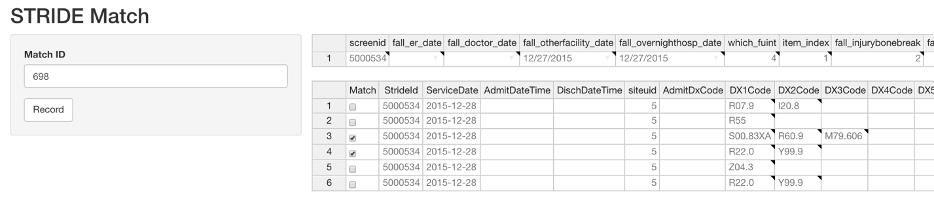
\includegraphics[width=\textwidth]{ui-1.png} 
\caption{Current User Interface}\label{fig:unnamed-chunk-1}
\end{center}
\end{figure}

To get information about a particular subject, users can enter the
subject ID in the left box and click the ``Record'' button. Our shiny
app will then display basic information about the subject in the top
right, and all stride records associated with the subject in the bottom
right. For instance, if the user searches for subject 698, our app will
display six stride records related to that subject. Each record has a
``match'' option, which our model uses to predict whether the record
matches our needs. If a record is ticked, it means our model has
predicted it to be a match. In the example shown in the figure, the
subject has two stride records that match our requirements. Users can
also manually tick the ``match'' column to mark a record as a match, and
the results will be stored in our database automatically to improve the
model's performance.

However, there are some errors that occur when searching for specific
subjects. For example, if we search for id=712, our shiny app cannot
fetch the stride record table for this person, and thus errors are
displayed directly on our front-end as follows. This may confuse our
users as they may not be aware of its meaning. Therefore, we need to
dive deep into our back-end and database to figure out the source for
this kind of error. If the error is unavoidable, we will use an alarm or
messages to make it more clear and concise for our users.

\begin{figure}[h]
\begin{center}
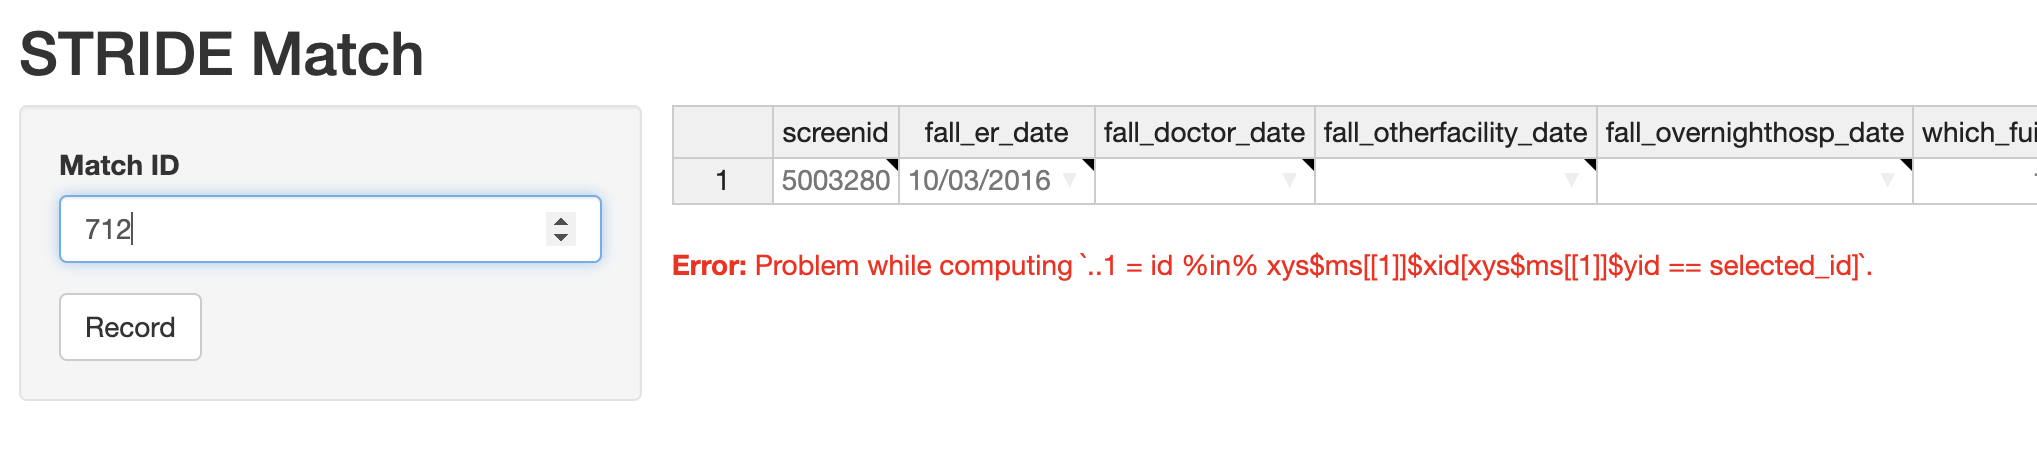
\includegraphics[width=\textwidth]{ui-2.png} 
\caption{Current User Interface (Error)}\label{fig:unnamed-chunk-2}
\end{center}
\end{figure}

\paragraph{Experimental Approach:}\label{experimental-approach}

In order to enhance the functionality of our shiny application, we will
develop several application features using the R programming language to
perform a wider variety of tasks and improve the overall user
experience.

\begin{itemize}
\tightlist
\item
  We will be introducing a ``capture new check'' feature that will
  enable users to create a new check within the application. This
  feature will provide users with greater flexibility in how they use
  the application and will make it easier for them to track and manage
  their progress.
\item
  We will add a ``note text box'' feature that will allow users to add
  notes to their work as they progress through the application. This
  feature will help users to stay organized and will make it easier for
  them to remember important details as they work.
\item
  In addition to these features, we will be introducing ``next'' and
  ``previous'' match buttons that will allow users to navigate through
  their work more easily. This feature will be particularly useful for
  users who are working on larger projects and need to move quickly
  between different parts of the application.
\item
  We will dive deep into the current shiny application and develop a
  comprehensive testing plan that includes several unit tests. These
  tests will be designed to identify any bugs or errors that may be
  present in the application, and will help us to ensure that the app is
  delivered to users in a bug-free state.
\end{itemize}

By using these experimental techniques to develop new features in our
shiny application, we hope to improve the overall user experience and
make the application more versatile and useful to users.

\paragraph{Interpretation of Results:}\label{interpretation-of-results}

Our designed user interface is displayed below.

\begin{figure}[h]
\centering
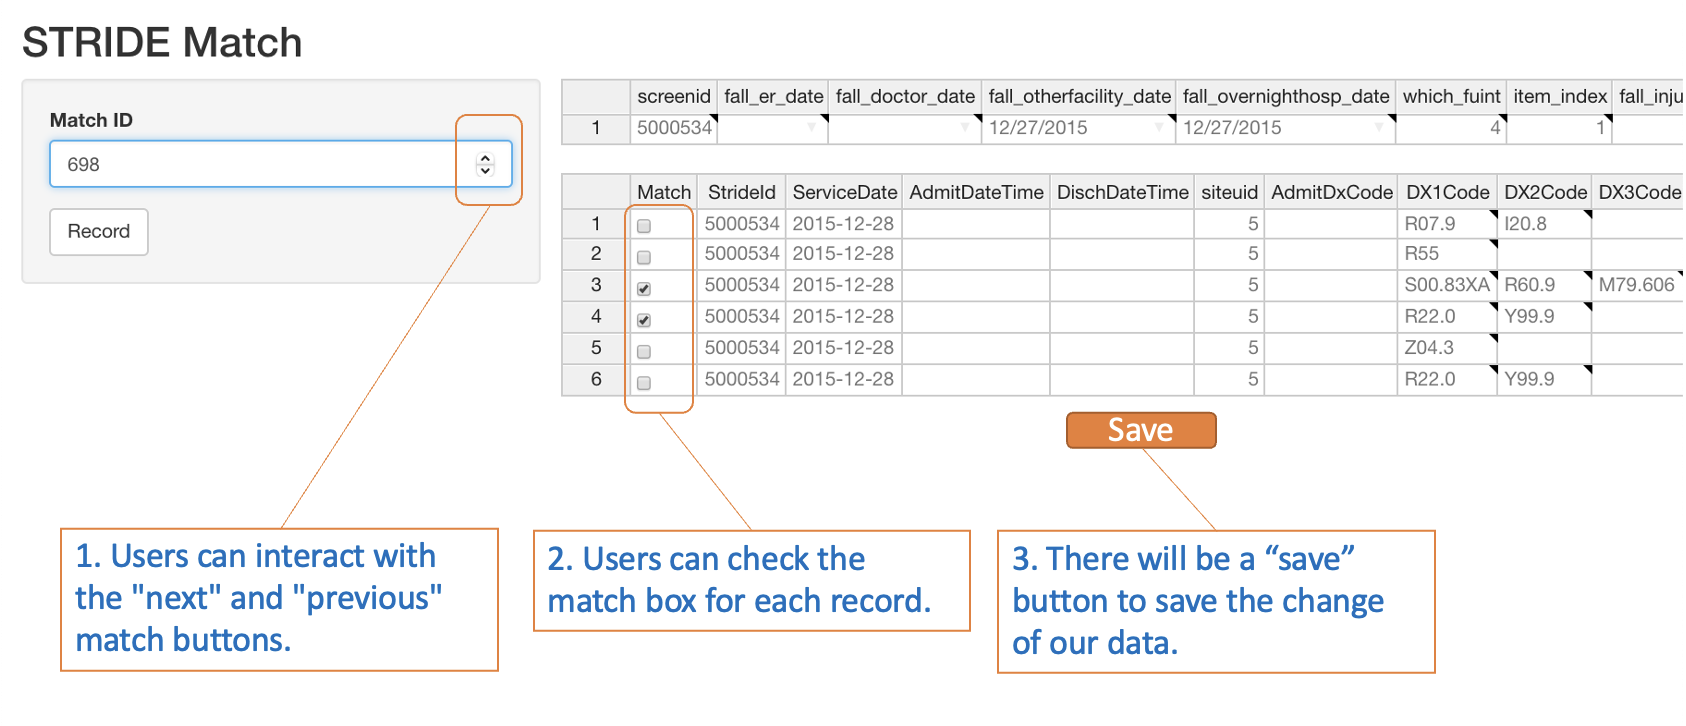
\includegraphics[width=0.9\textwidth]{ui-3.png} 
\caption{Designed User Interface}\label{fig:unnamed-chunk-3}
\end{figure}

\paragraph{Potential Problems and Alternative
Approaches:}\label{potential-problems-and-alternative-approaches}

As we go through our development process, it's possible that we may
encounter some issues.

\begin{itemize}
\tightlist
\item
  The first feature we are introducing is the ``capture new check''
  feature. While this feature provides users with greater flexibility
  and the ability to track and manage their progress more easily, it
  also presents potential issues with data privacy and security. To
  address these concerns, we will need to ensure that user data is
  securely stored and encrypted, and that only authorized users have
  access to it. Additionally, we will need to carefully consider how
  this feature is integrated into the overall application design and
  user interface, to ensure that it is easy to use.
\item
  The second feature we are introducing is the ``note text box''
  feature. While this feature provides users with a useful tool for
  staying organized and remembering important details, it may also
  present challenges with information overload and cluttered user
  interface. To address these concerns, we will need to carefully
  consider how notes are stored and displayed within the application,
  and provide users with the ability to easily manage and organize their
  notes as needed.
\item
  The third feature we are introducing is the ``next'' and ``previous''
  match buttons, which will allow users to navigate through their work
  more easily. While this feature provides users with greater
  convenience and efficiency, it may also present challenges with
  information overload and navigation complexity. To address these
  concerns, we will need to carefully consider how the buttons are
  integrated into the overall application design and user interface, and
  provide users with the ability to customize their navigation
  preferences as needed.
\item
  Finally, our comprehensive testing plan presents its own set of
  potential problems and alternative approaches. While unit tests are an
  effective tool for identifying bugs and errors in the application,
  they may not capture all potential issues that users may encounter in
  real-world scenarios. To address this concern, we will need to
  supplement our unit tests and gather feedback from a diverse range of
  users to ensure that the application meets the needs and expectations
  of its target audience.
\end{itemize}

In conclusion, the four features we are introducing, along with our
testing plan, present potential challenges that need to be carefully
evaluated and addressed to ensure the success of our shiny application.
By taking a thoughtful and strategic approach to the development and
testing process, we can overcome these challenges and deliver an
application that is intuitive, user-friendly, and bug-free.

\paragraph{\texorpdfstring{\textbf{Specific Aim 2: Develop matching
algorithm.}}{Specific Aim 2: Develop matching algorithm.}}\label{specific-aim-2-develop-matching-algorithm.}

\paragraph{Hypothesis:}\label{hypothesis-1}

Our hypothesis is that by using machine learning and deep learning
methods, we can develop a match algorithm that can accurately and
efficiently match EHRs with insurance

\paragraph{Rationale:}\label{rationale-1}

Manual matching between the EHRs and insurance records is a complex and
labor-intensive task that requires experienced staff. By automating the
matching process, we can reduce the time and effort required to match
records, while also improving the accuracy of the matching. This will
help to improve the overall efficiency of the healthcare system and
provide better care to patients.

We plan to randomly split our preprocessed data into three parts: train,
validate and test. We will use our train data to train the model, in
other words, to derive the appropriate parameters/model to fit the data.
And we will tune our hyper-parameters based on observation on the
performance of the validation data. Last, we test our model on the test
data, which is part of our full data, but has no relation with our
choice of the model/parameters. So it is the optimal choice to test our
model on the test data.

\paragraph{Experimental Approach:}\label{experimental-approach-1}

Suppose the insurance record and EHR pairs are our observations Xs, and
matching or not is the response which has only two values. So we
transformed our task to a binary classification problem.

To test our hypothesis, we plan to explore two directions: traditional
machine learning methods and deep learning methods. The experimental
approach will involve the following steps:

\begin{itemize}
\tightlist
\item
  \textbf{Data cleaning and preprocessing}: We will clean and preprocess
  the data to get rid of outliers, contaminated records, and do feature
  selection if necessary.
\item
  \textbf{Data splitting}: We will randomly split our preprocessed data
  into three parts: train, validate and test.
\item
  \textbf{Data statistics}: We will collect the specific statistics of
  our preprocessed data, such as the distribution of the Xs and Ys to
  check if the label is balanced. If not, we will further do
  up/down-sampling to prepare for our model.
\item
  \textbf{Model selection}: We will do experiments on both traditional
  machine learning models such as logistic regression, decision tree,
  and random forest, and deep learning models such as neural networks.
  We will try various combinations of layers and models depending on the
  data statistics and network performance.
\item
  \textbf{Performance evaluation}: We will use the accuracy and ROC/AUC
  metric to evaluate our model performance. We will also compare the
  performance of the traditional machine learning models and deep
  learning models.
\end{itemize}

\paragraph{Interpretation of
Results:}\label{interpretation-of-results-1}

The accuracy and ROC/AUC metric will be used to evaluate the performance
of our model. Accuracy is simply the percentage of the correct
predictions, which is limited when the data is imbalanced. So we use
ROC/AUC score. It tells us how efficient the model is. The higher the
AUC, the better the model's performance at distinguishing between the
positive and negative classes. An AUC score of 1 means the classifier
can perfectly distinguish between the classes, which is, if they match
or not.

\paragraph{Potential Problems and Alternative
Approaches:}\label{potential-problems-and-alternative-approaches-1}

One potential problem we foresee is how the raw data can be encoded to
machine learnable features properly. Based on our preliminary research
on the data, it is quite noisy mixed with null values, natural language,
characters and numbers. It can be tough if the features cannot be
embedded very well and it will definitely affect the model performance.
To solve this challenge, we aim to find the patterns beneath the data
and will try various encoding methods on it, including pre-trained
embeddings although we know transfer learning is hard to do.

\bibliography{references.bib}


\end{document}
